\documentclass[main.tex]{subfiles}

\begin{document}
    \chapter[The Influence of Hydrogen Envelopes in the Evolution of Partially-Stripped Helium Stars]{The Influence of Hydrogen Envelopes in the Evolution of Partially-Stripped Helium Stars}

    \begin{center}
        \textbf{S. Chanlaridis} and J. Antoniadis \\
    \end{center}

    % \textbf{Disclaimer:} This Chapter presents preliminary results from ongoing research that have not yet been subjected to peer review or published in any preprint format. As such, the findings and interpretations discussed in this chapter should be considered provisional and may be subject to revision. The results presented here are part of an ongoing investigation, and further analysis and validation are required before any definitive conclusions can be drawn.
        
        
    \begin{center}
        \textbf{\large Abstract}
    \end{center}
    
    The majority of massive stars are born in binary or multiple systems, where, in most cases, the stars will eventually undergo a phase of mass transfer. During this phase, the gravitational force of one star (the accretor) strips material away from its companion (the donor). 
    The extent to which the donor loses its hydrogen envelope depends on numerous factors known to affect the efficiency of envelope stripping in such interacting binaries (e.g., convective overshooting, semiconvective and rotational mixing). In some instances, the stripping process is incomplete, leaving the star only partially stripped, with a thin layer of hydrogen still surrounding its exposed inner layers. Depending on the remaining hydrogen and the star’s internal structure, they may follow distinct evolutionary paths: they may either undergo core-collapse, leading to neutron star formation, or trigger thermonuclear explosions.

    In this work we investigate the importance of residual hydrogen in the envelopes of helium stars for their evolution and final fate. In particular, this work seeks to determine the threshold of leftover hydrogen that allows these stars to undergo explosive oxygen ignition at relatively low densities, as it has recently been demonstrated.

    We perform numerical calculations to model the evolution of partially stripped, low-mass helium stars at solar metallicity. 
    We find that the presence of hydrogen-polluted envelopes can significantly alter the final fates of low mass, stripped helium stars. A hydrogen mass of $0.5\msun$ suffices to maintain hot bottom burning for long enough so that the evolution is accelerated, leaving behind an oxygen-neon white dwarf with a significant amount of residual carbon distributed within its core. In contrast, lower hydrogen mass has no significant influence, as it is rapidly exhausted, leading to explosive oxygen burning.

    Depending on the degree of mass loss, inefficient stripping of intermediate mass stars in binaries may naturally lead to the formation of oxygen-neon white dwarfs harboring a significant amount of residual carbon. These compact objects may be prone to disruption as subsequent mass transfer onto the white dwarf's surface may trigger carbon ignition, leading to a thermonuclear runaway and having a negative impact on the neutron star formation rate via accretion-induced collapse.
    
    
    {\hypersetup{linkcolor=black, pdfborder={0 0 0}}
        \minitoc
        \newpage
    }
    
    \section{Introduction} \label{sec:ch3:intro}
    Hydrogen-deficient stars, characterized by their low surface hydrogen content, present intriguing cases for stellar astrophysics. They are often associated with advanced stages of stellar evolution, where significant mass loss reveals inner, helium-rich layers. The formation of these stars is believed to be heavily influenced by binary evolution, either through stable mass transfer or common-envelope (CE) events \citep[e.g.,][]{2008ASPC..391..221D, 2008ASPC..391..323P}. These channels are both critical in stripping the hydrogen envelope from an evolving star, exposing deeper, processed layers primarily composed of helium and other fusion products.

    In binary systems, mass transfer can occur in a stable manner if the mass-losing star transfers material to a companion at a manageable rate, typically while the donor star is still on the red-giant or asymptotic-giant branch. This stable Roche lobe overflow (RLOF) scenario allows for the gradual removal of the donor’s hydrogen envelope, exposing the helium core and transforming the star into a hydrogen-deficient object. Stable transfer, however, requires a mass ratio and orbital configuration that prevent runaway transfer, where the donor’s rapid expansion would lead to a CE and a spiral-in phase. 

    In contrast, CE evolution represents a more dramatic and often catastrophic event in binary systems. During CE evolution, the expanding donor’s envelope engulfs the companion, leading to intense frictional drag within the envelope and a rapid loss of angular momentum. This event causes the envelope to be ejected, leaving a close binary of the stripped helium core and its companion. While CE events are complex and not fully understood, they are considered essential to the formation of many hydrogen-deficient stellar types, including helium stars (He stars), subdwarf B-stars, and even some progenitors of type Ia supernovae (\ias). In particular, recent studies have shown that fully stripped He stars may evolve into highly degenerate oxygen-neon (ONe) cores and subsequently explode in \ia-like events \citep{AC20, CA22}. The trigger mechanism, in this case, may be the ignition of leftover carbon from incomplete off-center carbon burning. 

    In this work, we build detailed numerical models to study the effects of residual hydrogen envelopes in the evolution of partially stripped He stars. The text is organized as follows: in Sect.~\ref{sec:ch3:methods} we describe our models and the physical assumptions. In Sect.~\ref{sec:ch3:results} we present the results of our simulations and in Sect.~\ref{sec:ch3:discussion} we conclude with a discussion on the ramifications of our models and future research.

    \section{Numerical calculations} \label{sec:ch3:methods}
    We performed our numerical simulations using the implicit one-dimensional code \textbf{M}odules for \textbf{E}xperiments in \textbf{S}tellar \textbf{A}strophysics \citep[\mesa\,v10398;][]{Paxton:2010ji,Paxton:2013pj,Paxton:2015jva,Paxton:2017eie}.
    % Description of our models
    We followed the evolution of two models, \textsc{h0p25} and \textsc{h0p5}, with residual hydrogen masses of $0.25\msun$ and $0.5\msun$, respectively. To this end, we began by tracking the evolution of $10\msun$ nonrotating, pre-main-sequence (pre-MS) stars until central hydrogen depletion. At this point, we imposed an artificial wind of $10^{-3}\mdotsun$ to mimic a rapid mass transfer phase that reduces the H-rich surface material up to a user-specified hydrogen mass. The resulting stripped stars are assumed to not participate in any further binary interactions and are allowed to continue their evolution without employing any physical stopping conditions. All other physical assumptions are similar to those described in \cite{AC20} and \cite{CA22}. Here, we only briefly summarize them for completeness.
    
    The initial pre-MS models have a uniform composition with $X=0.7$, $Y=0.28$, and $Z=0.02$. Convection was treated using the mixing-length theory \citep[MLT;][]{MLT_Henyey}, with the Ledoux criterion applied to assess convective stability \citep{Ledoux:apj1947}. A mixing-length parameter of $\alpha_{\rm ML}=2.0$ was selected. To enhance the efficiency of convective energy transport, the \texttt{MLT++} variant of the standard MLT, available in \mesa, was used, which reduces the superadiabatic gradient \citep{Paxton:2015jva}. Additional internal mixing processes, such as thermohaline and semiconvection, were included and treated as diffusive processes. In both cases, the mixing parameters were taken to be $\alpha_{\rm SEM} = D_{\rm TH} = 1.0$ \citep{Langer1991, Brown_2013}. Predictive mixing and overshooting beyond convective boundaries were not considered in any of our models.
    
    Our nuclear reaction network included 43 isotopes and accounted for all significant weak interactions, using weak reaction rates from \cite{Suzuki2016}. Corrections for ion and electron screening were applied following the work of \cite{PCR2009} and \cite{Itoh2002}, respectively. Opacity data were sourced from type-2 OPAL opacity tables \citep{OPAL}. For mass loss due to stellar winds, we implemented the \texttt{Dutch} wind scheme \citep{Dutch}. Specifically, for temperatures $T_{\rm eff} > 10^4$\,K and a surface abundance of hydrogen of $X < 0.4$ by mass fraction, the mass-loss rate followed the prescription from \cite{Nugis2000} with a scaling factor of $\eta = 1$. For $T_{\rm eff} < 10^4$\,K we used the mass-loss prescription of \cite{deJager1988}. 

    \section{Results}\label{sec:ch3:results}
    After the depletion of hydrogen in the core, energy generation shifts to a hydrogen-burning shell surrounding the inert helium core. This shell burning, driven by the CNO cycle, produces substantial energy, leading to the formation of a convective region that facilitates the mixing of chemical elements. As the core contracts and heats up, the helium core grows in mass while the hydrogen-burning shell slowly moves outward. Simultaneously, the radius of the star increases as it ascends the red giant branch. It is at this stage that we assume that the star undergoes a significant stripping event, losing much of its outer hydrogen envelope. Our two models relax to a new initial mass of approximately $2.4\msun$ and $2.9\msun$ for models \textsc{h0p25} and \textsc{h0p5}, respectively.
    This stripping dramatically alters the stars' structure, reducing the pressure on the outer layers and exposing regions closer to the hydrogen-burning shell. Figure~\ref{fig:kipp_plots} shows Kippenhahn diagrams that capture the structural evolution of the star after the initial hydrogen depletion in the core and subsequent stripping of its envelope. The horizontal axis shows the logarithmic time before the end of the simulation in years, while the vertical axis indicates the mass coordinate within the star in solar masses. The color scale represents the net energy generation, distinguishing between regions where energy is generated (red) and lost (blue), primarily through nuclear reactions and neutrino cooling. The orange and green hatching indicates thermohaline and convective regions, which play a key role in mixing material within the star. 

    \begin{figure*}
        \centering
        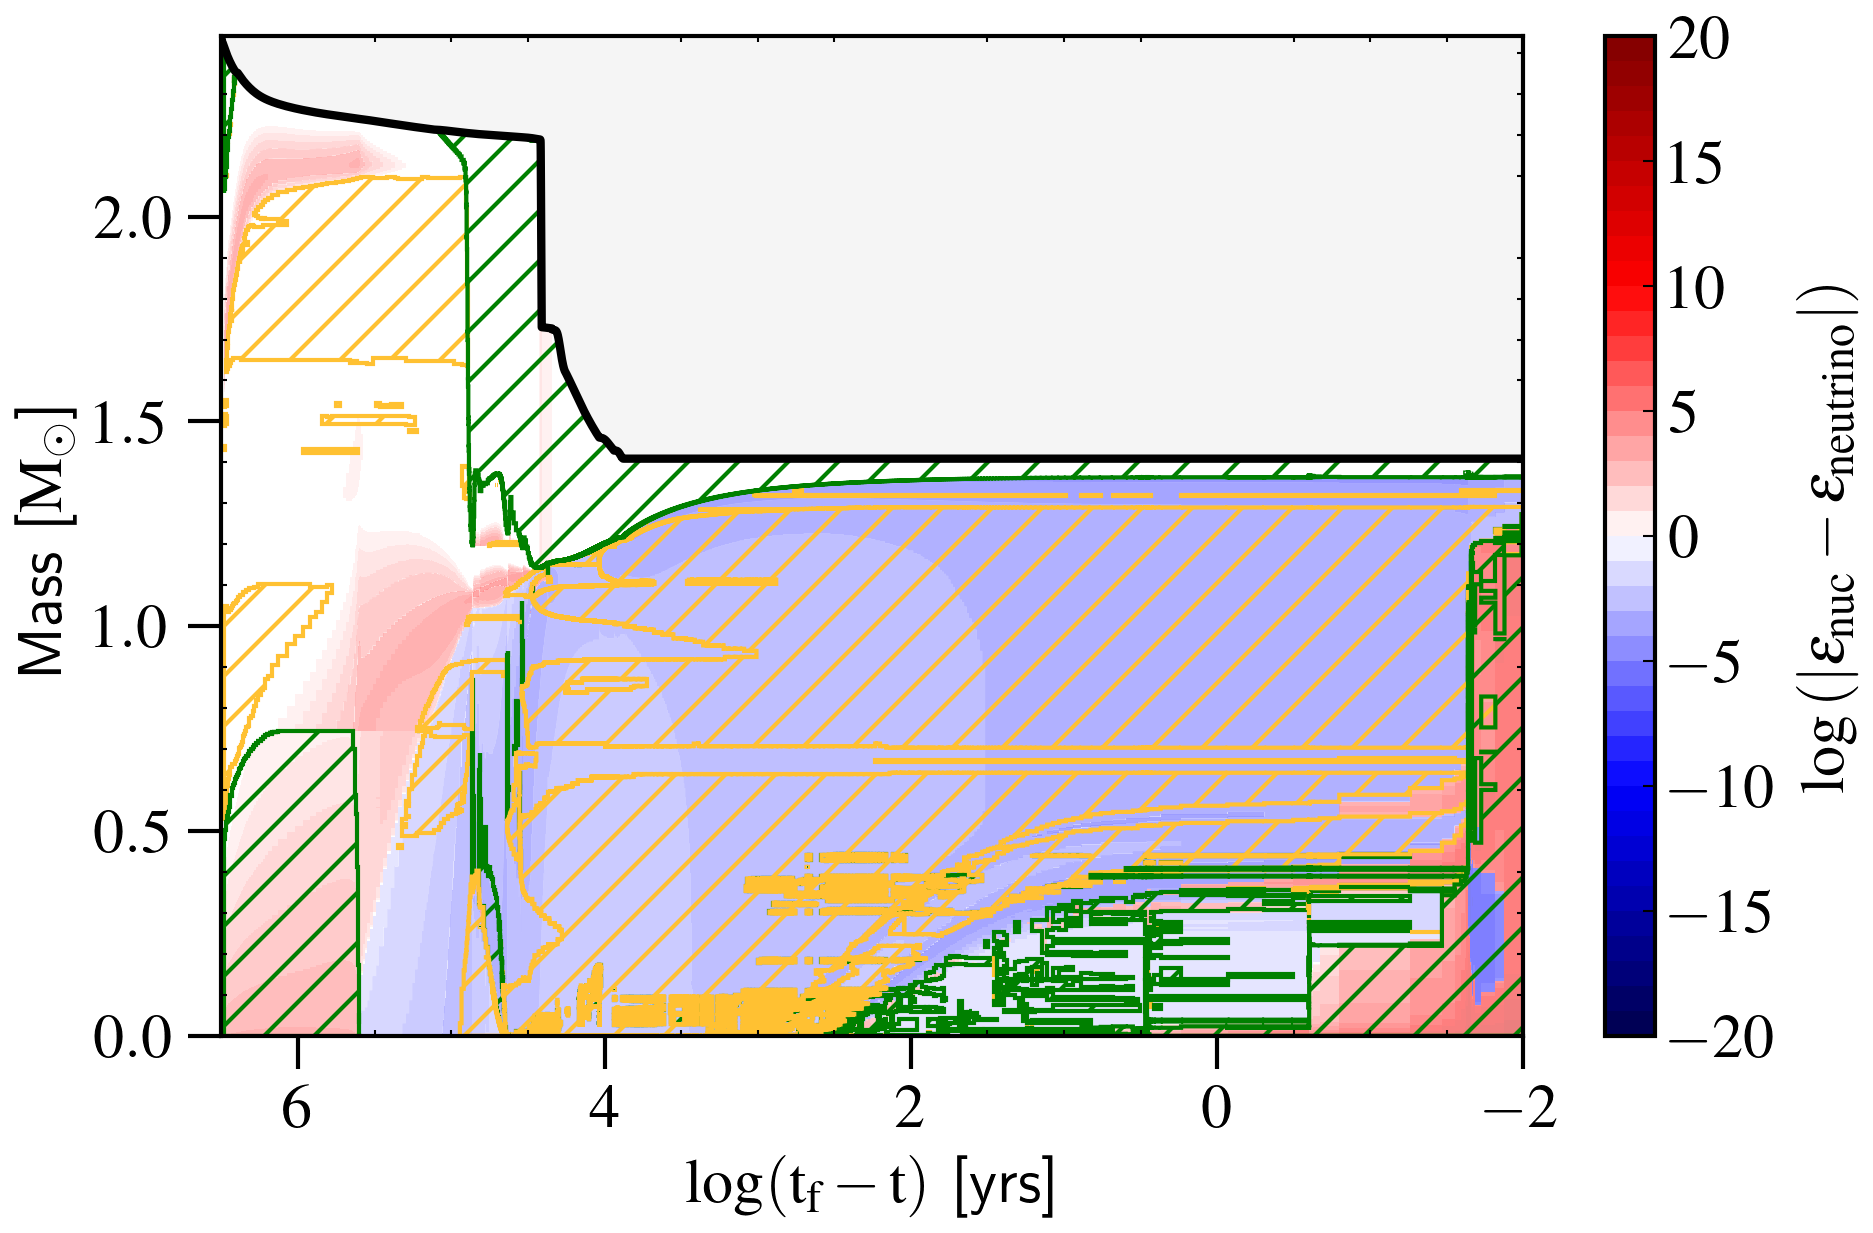
\includegraphics[width=0.45\textwidth]{figures/chapter3/kipp_H0p25.png}
        \hspace{0.5cm}
        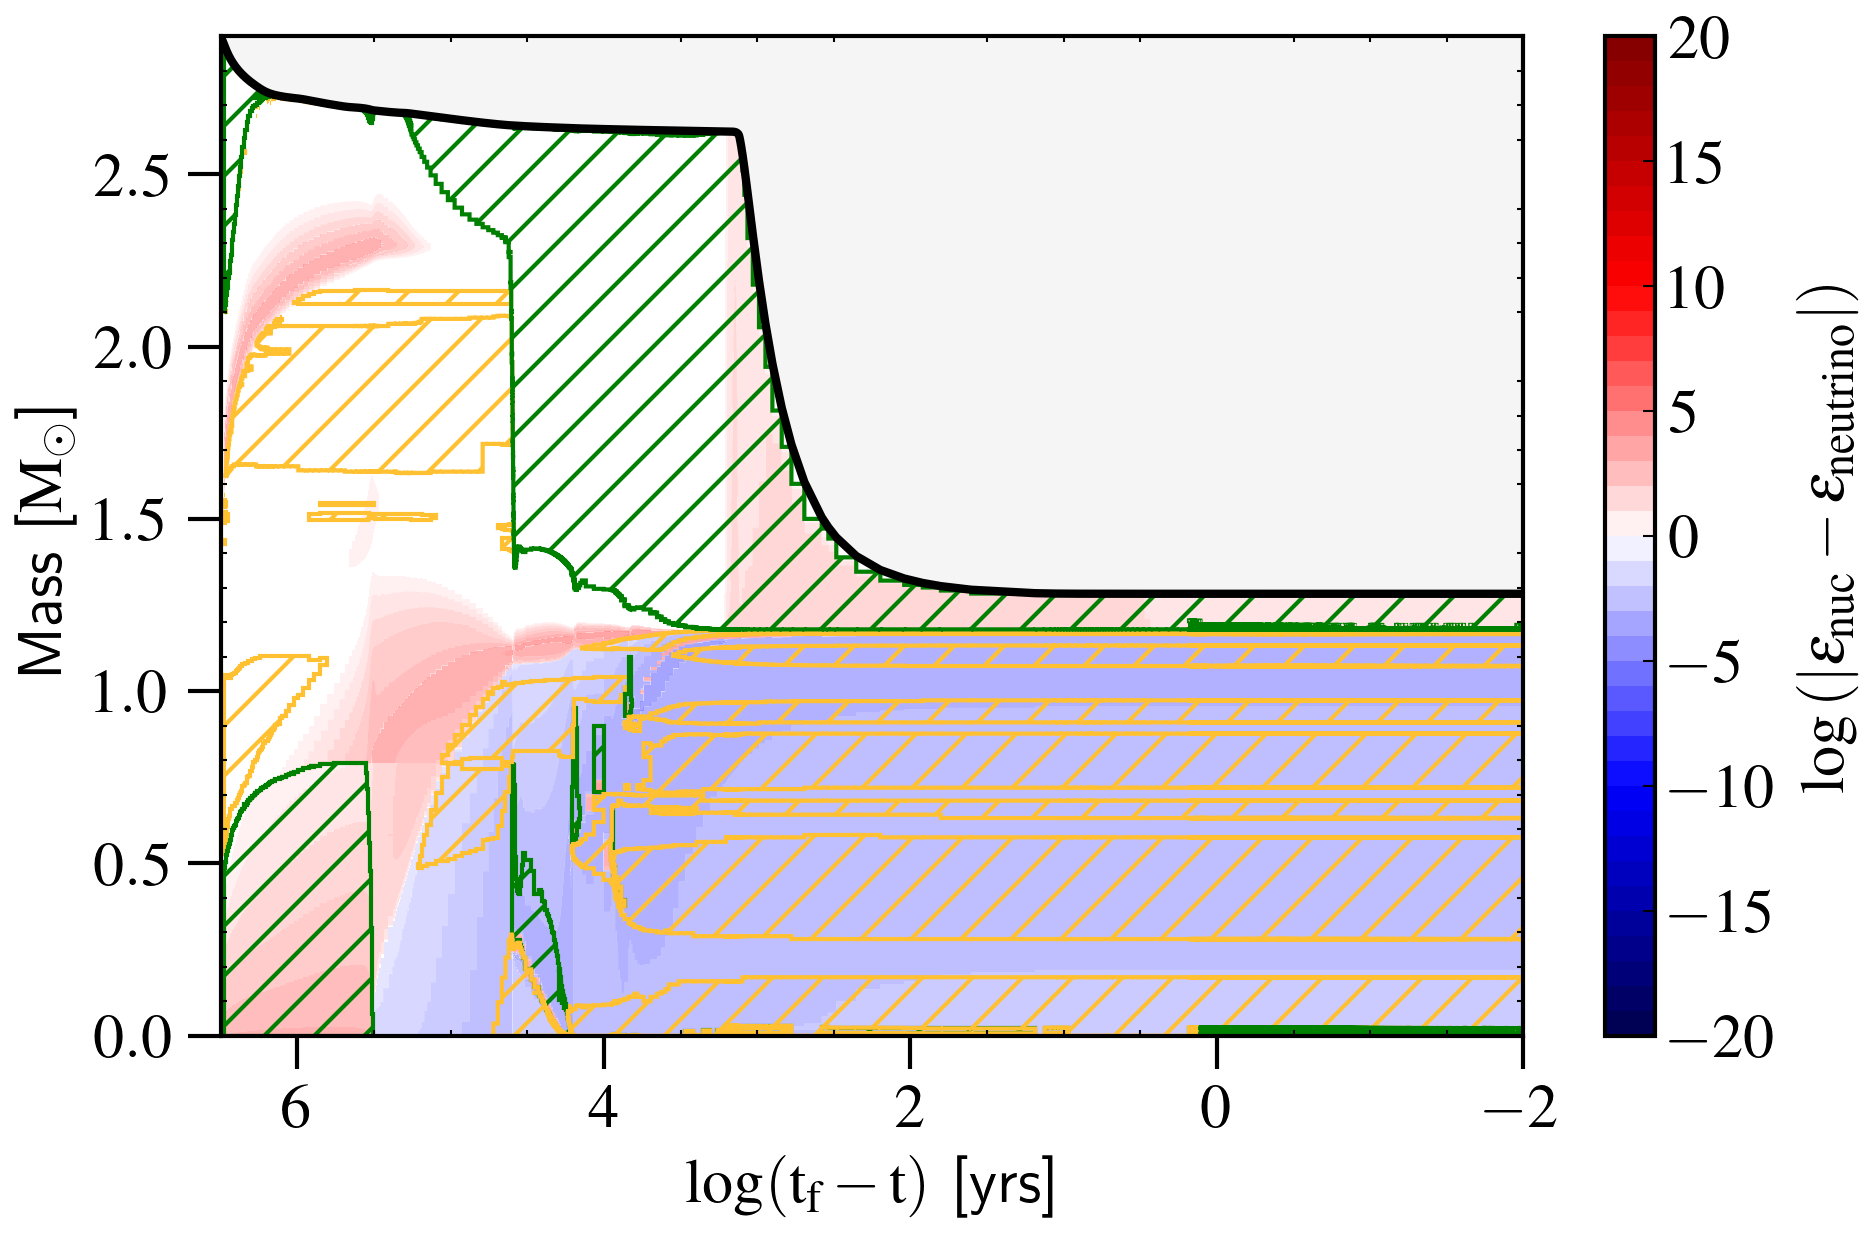
\includegraphics[width=0.45\textwidth]{figures/chapter3/kipp_H0p5.png}
        \caption{Kippenhahn diagrams for models \textsc{h0p25} (left) and \textsc{h0p5} (right) as a function of remaining evolution time after initial stripping. Green and gold hatched areas denote convection and thermohaline mixing respectively. The colorbar indicate net energy rate.}
        \label{fig:kipp_plots}
    \end{figure*}
    
    Following the envelope stripping, the star adjusts to its reduced mass, settling into a configuration where the remaining hydrogen-rich outer layers sustain energy generation through shell hydrogen burning. This shell is visible as a narrow region of energy generation above the growing helium core. The core itself begins helium burning, through the triple-alpha process, shortly after hydrogen shell burning is established, producing carbon and oxygen (CO) and creating a convective core. 
    
    As helium in the core becomes depleted ($\log(t_{\rm f} - t) \simeq 5.5$), the energy source shifts to a helium-burning shell that surrounds the CO core. The core itself becomes inert and degenerate. Over time, the core cools through significant neutrino losses, as indicated by the blue shading in the inner regions. Meanwhile, hydrogen burning persists in a shell closer to the surface, driving mass accretion onto the helium-burning shell below.
    
    At later stages ($\log(t_{\rm f} - t) \simeq 5$), off-center carbon ignition occurs in the degenerate CO core. This initiates a carbon-burning front that propagates inward, converting the core into an ONe composition. Convection extends deeply into the star during this phase, as indicated by the green hatched regions, bringing fresh hydrogen-rich material into the burning regions and briefly re-igniting hydrogen burning in the shell. In some cases, it can penetrate regions near the helium-burning shell, where residual hydrogen is ingested into the hot helium-burning layer. This interaction triggers a burst of energy as the ingested hydrogen undergoes rapid fusion in the extremely high-temperature environment. For the next circa 1000 yr, the increased surface luminosity ($L\simeq 10^{6.6}\lsun$) causes a sustained fast stellar wind that results in an enhanced mass loss with a maximum rate of $\sim 10^{-2.8}\mdotsun$. 
    
    \begin{figure*}
        \centering
        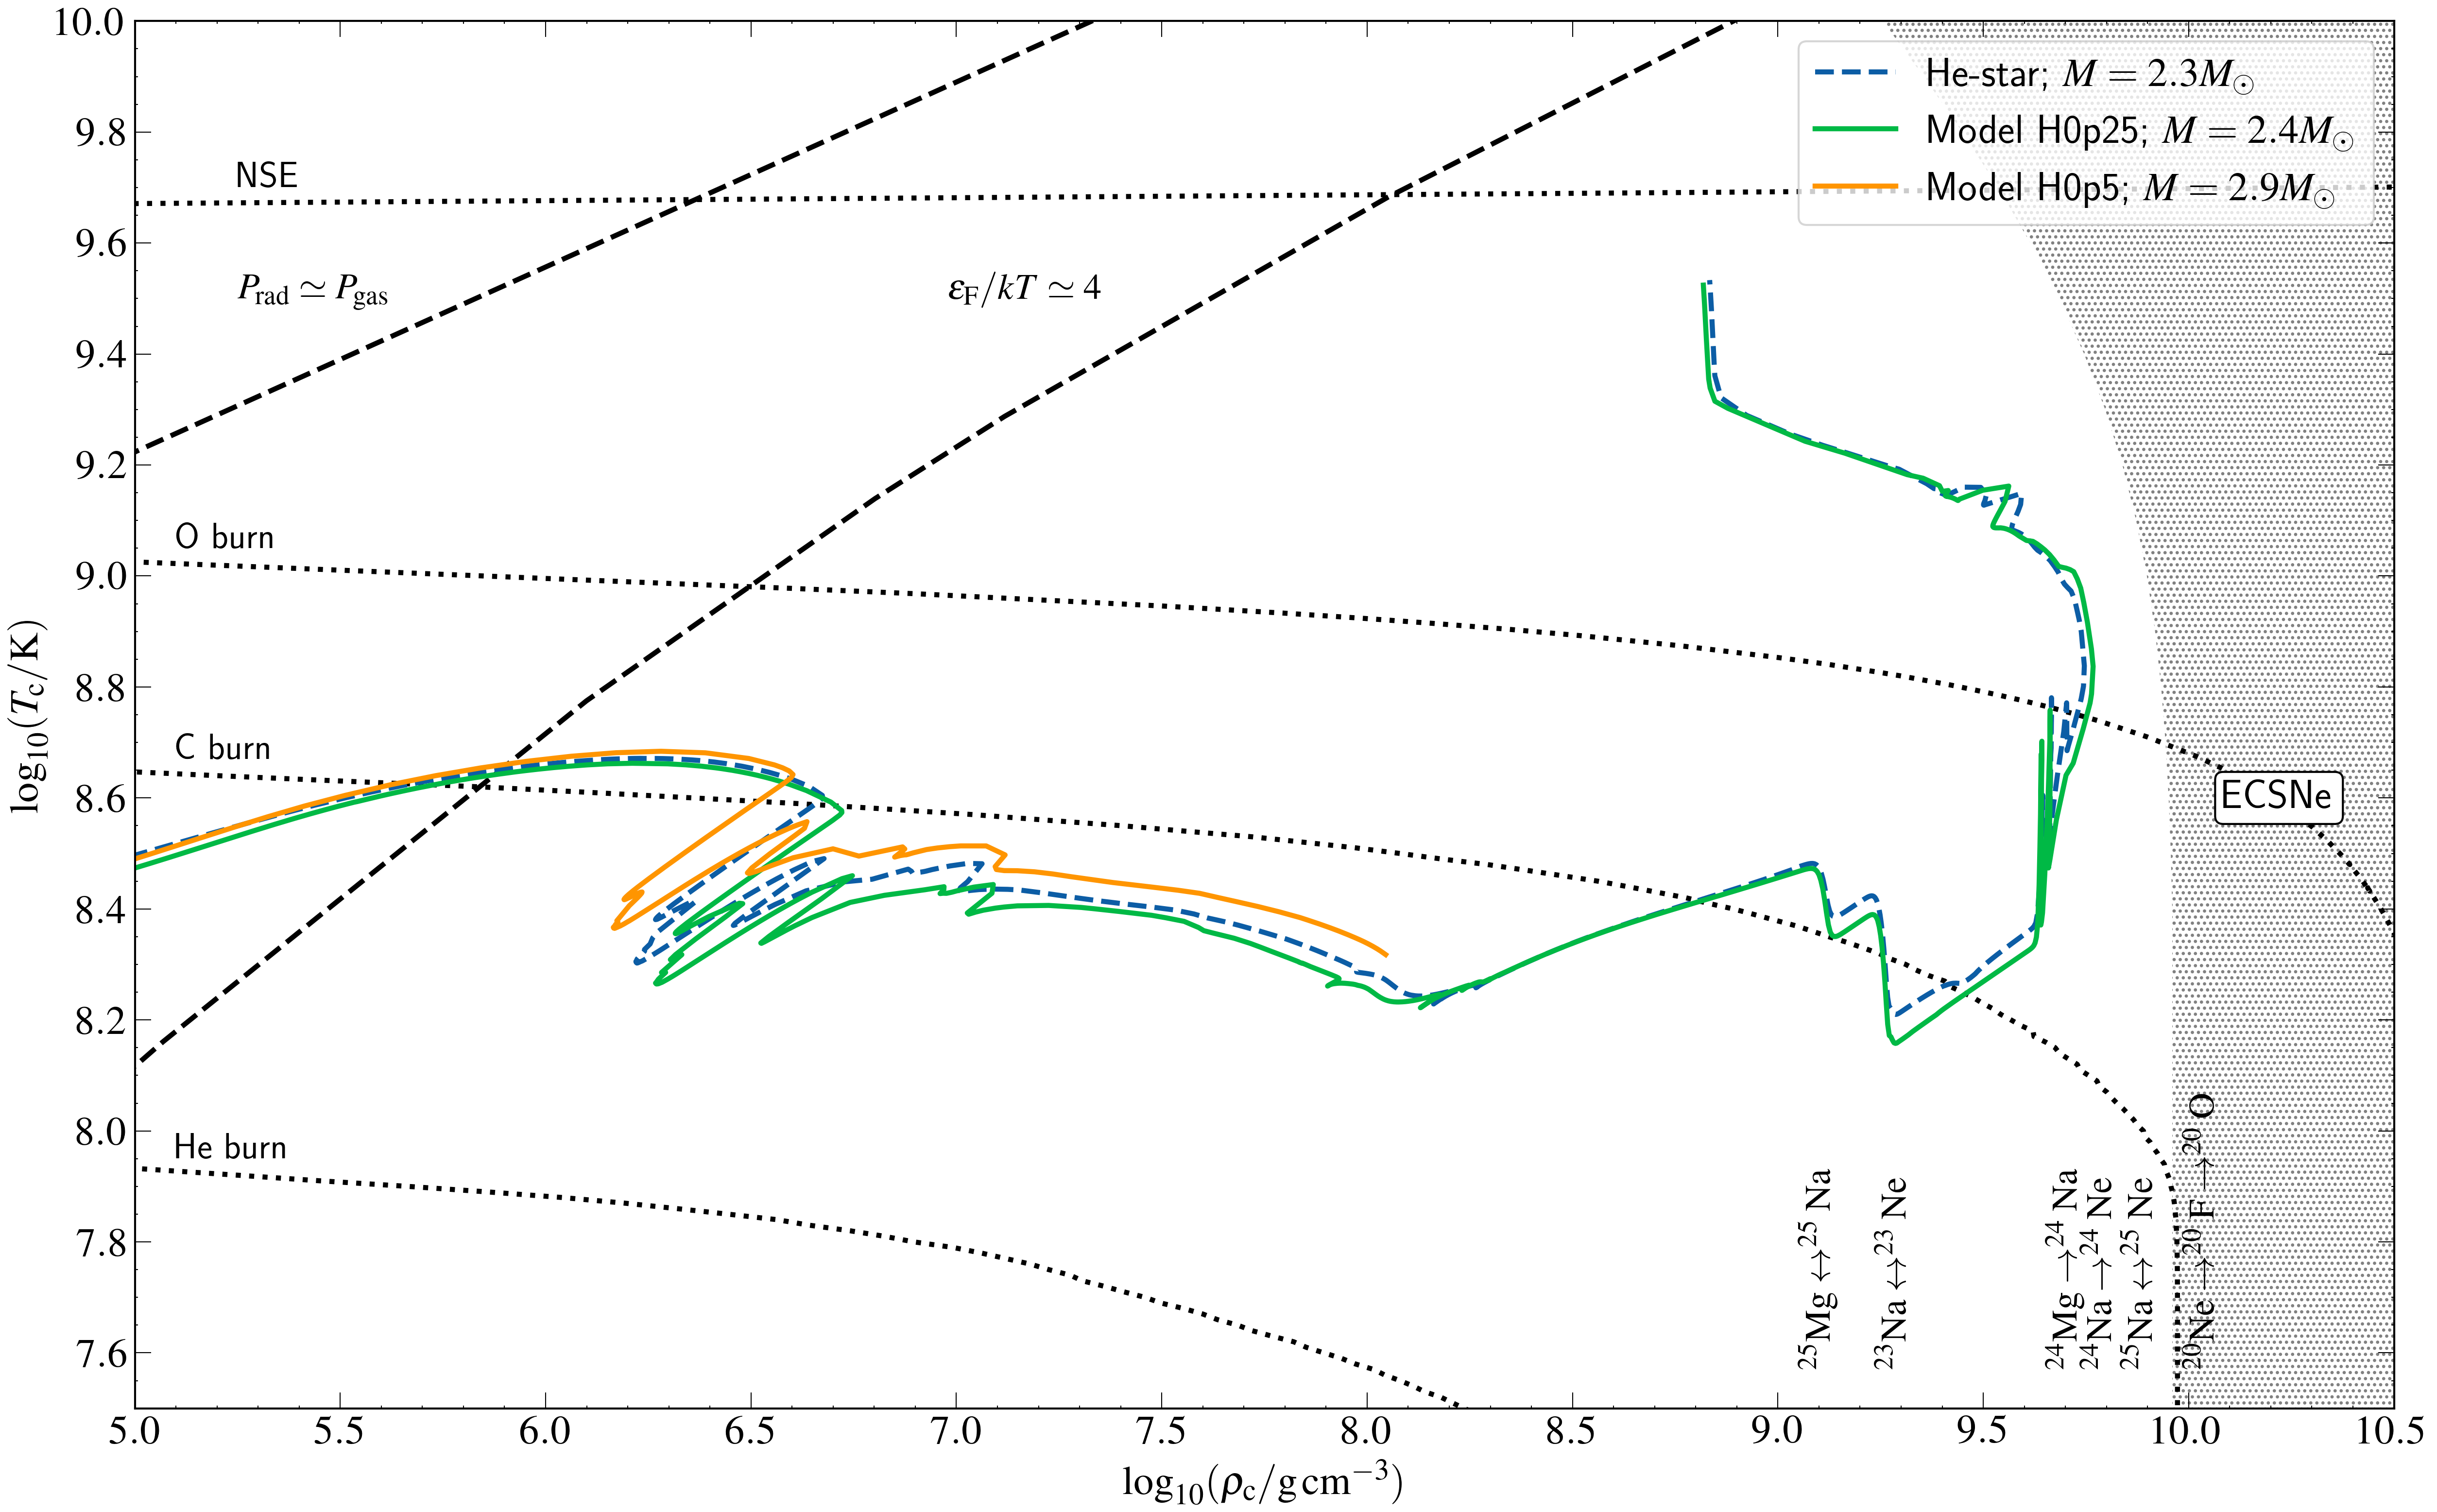
\includegraphics[width=0.8\textwidth]{figures/chapter3/rho_vs_temp.png}
        \caption{Evolution of the core density and temperature for models \textsc{h0p25} and \textsc{h0p5}. The dashed black line shows the approximate boundary for electron degeneracy.}
        \label{fig:rho_vs_temp_plot}
    \end{figure*}
    
    In both cases, following the completion of carbon burning, the cores of the models retain traces of unburned carbon, and their overall structural evolution aligns closely with the predictions from \cite{AC20} and \cite{CA22}. This evolution is illustrated in Fig.~\ref{fig:rho_vs_temp_plot}, which shows the trajectory of the cores in the central density-temperature plane. The solid green line represents the core evolution of model \textsc{h0p25}. Because this model retains only a small amount of hydrogen in its envelope, it does not undergo an extended phase of intense mass loss. Instead, the residual hydrogen is rapidly consumed, leaving the core to evolve as a hydrogen-free helium star. As the core contracts and heats up, its evolution closely mirrors that of a $2.3\msun$ helium star model (dashed blue line) from \cite{CA22}, which has solar metallicity and no overshooting. 
    As the density increases beyond $\log(\rho_c) \simeq 9.0$, weak Urca reactions, involving isotopes such as \iso{Mg}{25} and \iso{Na}{23}, begin to dominate. These reactions produce neutrinos, leading to cooling in the core. However, localized heating from these same reactions also creates conditions favorable for carbon re-ignition, which generates additional heat and raises the central temperature slightly. Both models reach the conditions for oxygen ignition at similar central densities and temperatures, ultimately leading to explosive oxygen burning at a relatively low density.
    
    In contrast, model \textsc{h0p5}, represented by the orange line in Fig.~\ref{fig:rho_vs_temp_plot}, contains enough residual hydrogen in its envelope to fuel continued hydrogen burning in a shell. This prolonged activity drives significant mass loss over time, stripping the star of its helium mantle and preventing the core from reaching the conditions necessary for explosive oxygen ignition. Instead, it forms an ONe white dwarf harboring a substantial amount of residual carbon having a mass average $X(\iso{C}{12}) \geq 0.004$. 

    \section{Discussion}\label{sec:ch3:discussion}
    The findings presented in this study offer a deeper understanding of the evolution and final outcomes of partially stripped He stars, illuminating their potential pathway toward thermonuclear explosions. Models with varying residual hydrogen masses demonstrate the critical role of hydrogen ingestion and mass loss in shaping the fate of these stars. Stars with minimal hydrogen envelopes, such as model \textsc{h0p25}, evolve as nearly hydrogen-free helium stars, resulting in core conditions favorable for oxygen ignition at relatively low densities, ultimately leading to thermonuclear explosions. By contrast, models retaining larger hydrogen envelopes, such as \textsc{h0p5}, experience prolonged shell burning and mass loss, stripping away their helium mantles and leaving behind ONe white dwarfs. These findings underscore the sensitivity of late-stage stellar evolution to envelope composition and residual hydrogen content, as these factors govern whether a star transitions to an explosive outcome or a degenerate remnant with leftover carbon distributed in its core.
    
    The evolution of such ONe cores featuring residual carbon presents a particularly interesting scenario requiring further investigation. Residual carbon distributed throughout the core can potentially influence the star’s explodability under the right thermodynamic conditions. As suggested by previous works, including \cite{AC20} and \cite{CA22}, compressional heating can trigger explosive oxygen ignition in hybrid CONe cores, whereas in ONe cores with residual carbon, electron captures on \iso{Mg}{24} nuclei play a pivotal role. These electron captures are highly sensitive to temperature and pressure, occurring only within specific (T, P) regimes. Once triggered, these reactions release sufficient energy to ignite the remaining carbon, initiating a cascade that culminates in oxygen ignition and a thermonuclear explosion. However, the spatial distribution of residual carbon within the core may critically influence this process, particularly in determining the timing and dynamics of the explosion. This can be especially important in cooling ONe white dwarfs where gravitational settling may re-distribute and alter the composition profile of the core. 
    In a binary system, mass transfer episodes onto the ONe white dwarf can significantly influence its evolution by driving the core toward conditions that either favor carbon ignition or lead to accretion-induced collapse (AIC) into a neutron star. 
    
    Two hypothetical scenarios can be considered regarding how the carbon distribution affects the outcome. In the first scenario, stars with carbon concentrated in their inner cores would experience earlier electron captures, as these regions are the first to achieve the necessary (T, P) conditions during gravitational compression. This early initiation of electron captures would favor such stars for explosions, as the outer layers of the core would still be compressing and contributing to the ignition sequence, preventing the AIC scenario. In contrast, stars with carbon concentrated in their outer cores would require the core to compress further for the outer regions to achieve the right conditions for electron captures. This delay might lead to conditions in the inner core surpassing those optimal for \iso{Mg}{24} electron captures, resulting in lower reaction rates and a postponed explosion. While this might still lead to detonation, the timing and dynamics of the event would differ, potentially altering the energetics and nucleosynthetic yields of the explosion.
    
    The second scenario considers the effects of a carbon distribution centered in the outer core. In this case, the inner core, with its low carbon abundance, might still achieve ignition under the right conditions, producing a subsonic burning front or shock wave. This front could propagate outward, compressing the outer layers of the core and accelerating their progression toward the (T, P) conditions required for electron captures. Such a scenario introduces the possibility of a faster, delayed detonation, where the initial carbon ignition indirectly facilitates the conditions for \iso{Mg}{24} reactions in the outer layers. However, the outcome could also differ significantly. Depending on the strength and dynamics of the burning front, the process could fail to sustain the necessary ignition conditions, leading to a failed thermonuclear explosion. This raises important questions about the interplay between the carbon distribution and the propagation of shocks or burning fronts within the ONe core.
    
    These considerations suggest that the spatial distribution of residual carbon has a profound impact on the evolutionary and explosive outcomes of ONe cores. 
    A centrally concentrated carbon profile is more likely to trigger early ignition, releasing energy that halts further compression and avoids collapse. Conversely, a carbon distribution skewed toward the outer layers must rely on the interplay between shock dynamics and delayed ignition to achieve a detonation, leaving the star at greater risk of collapsing into a neutron star if conditions are not ideal.
    
    Ultimately, the evolutionary fate of accreting ONe white dwarfs---whether they end in a thermonuclear explosion or undergo AIC---depends on the composition profiles, the accretion rate, and the thermal evolution of the core. 
    Future studies should investigate these dynamics in greater detail, including multidimensional simulations that account for asymmetries in burning and shock propagation. Such work will be crucial to illuminate the effects of carbon distribution, the conditions for detonation, and the nature of any resulting thermonuclear explosions.

\end{document}